\chapter{Metodología}

Para la realización del proyecto, la creación del videojuego, se dispondrán de 6 meses que se dividirán de la siguiente forma: inicialmente un mes y medio para la investigación, especificación del producto y planificación; cuatro meses desarrollando el producto; finalmente medio mes para dar los últimos retoques al juego y lanzar una versión beta.

Para el desarrollo del videojuego se utilizará una metodología ágil, ya que al disponer de poco tiempo para el desarrollo se necesitará tener un producto cuanto antes para poder enfrentarlo al público y obtener el feedback de este. Utilizando una metodología ágil se focaliza el esfuerzo en el desarrollo en lugar de en una excesiva planificación. De esta forma 
\begin{itquote}
	se trabaja realizando entregas parciales pero funcionales del producto. De ese modo, es posible entregar en el menor intervalo de tiempo posible una versión funcional del producto.
	\begin{flushright}
	 	\cite{eduardomartinez2014}.
 	\end{flushright}
\end{itquote}

Además la utilización de estas metodologías ayuda enormemente a reducir el riesgo: al crear un videojuego, en este caso educativo, a pesar de las mejores intenciones de los desarrolladores no se puede saber con certeza si será del agrado de los jugadores.

Es por ello que la mejor estrategia posible es crear un producto minimo viable (MVP) y que posteriormente se desarrolle y corrija según los deseos de aquellos que lo jugarán. 

Existen actualmente una gran cantidad de metodologías ágiles. Entre las más populares se pueden destacar: 

\begin{itemize}
	\item Scrum: es una metodología orientada a equipos. Proporciona herramientas para el seguimiento diario del proyecto, la planificación de trabajo de forma iterativa y la comunicación y cooperación de los integrantes del grupo.
	\item Extreme Programming: orientada a equipos con pocos programadores. 
		\begin{itquote}
			se aplica en equipos con muy pocos programadores quienes llevan muy pocos procesos en paralelo. Consiste entonces en diseñar, implementar y programar lo más rápido posible, hasta en casos se recomienda saltar la documentación y los procedimientos tradicionales.
			\begin{flushright}
	 			\cite{opheliapastrana2015}.
 			\end{flushright}
		\end{itquote}
	\item Kanban: esta metodología propone dividir el trabajo en diferentes etapas bien diferenciadas. El objetivo es evitar los cuellos de botella limitando el trabajo en curso. Para ello, se establece un límite de trabajo en curso, lo que obliga a que cuando una tarea se empieza se debe terminar antes de iniciar una nueva.
\end{itemize}

La metodología ágil a utilizar será Kanban ya que es tremendamente sencilla de implementar: con unas simples tarjetas se pueden especificar las tareas a realizar, y con un tablero se pueden crear columnas que representan los estados de las diferentes tareas.

Dada la facilidad con la que se puede implementar Kanban, y que no es un sistema directamente orientado a equipos como SCRUM, será muy adecuado para el proyecto.


En cuanto al producto a desarrollar, los cuatro meses de desarrollo se dividirán en iteraciones de duración variable. Al finalizar la segunda iteración se espera tener un mínimo producto viable (MVP) y en las dos siguientes se perfeccionará dicho producto.

En cuanto al tiempo de desarrollo se dividirá en cuatro iteraciones: 

\begin{itemize}
	\item Primera iteración: desarrollo de la parte software del MVP usando placeholders en lugar de los modelos 3D y los demás elementos gráficos
	\item Segunda iteración: inclusión de los modelos 3D e imágenes definitivas
	\item Tercera iteración: recolección de feedback y corrección de errores. Optimización del juego
	\item Cuarta iteración: recolección de feedback y corrección de errores. Detalles finales del juego
\end{itemize}

Para ilustrar esta distribución de tareas se ha creado un diagrama de Gantt simplificado como se puede apreciar en la siguiente imagen \ref{gantt01}.

\begin{figure}
	\begin{center}
		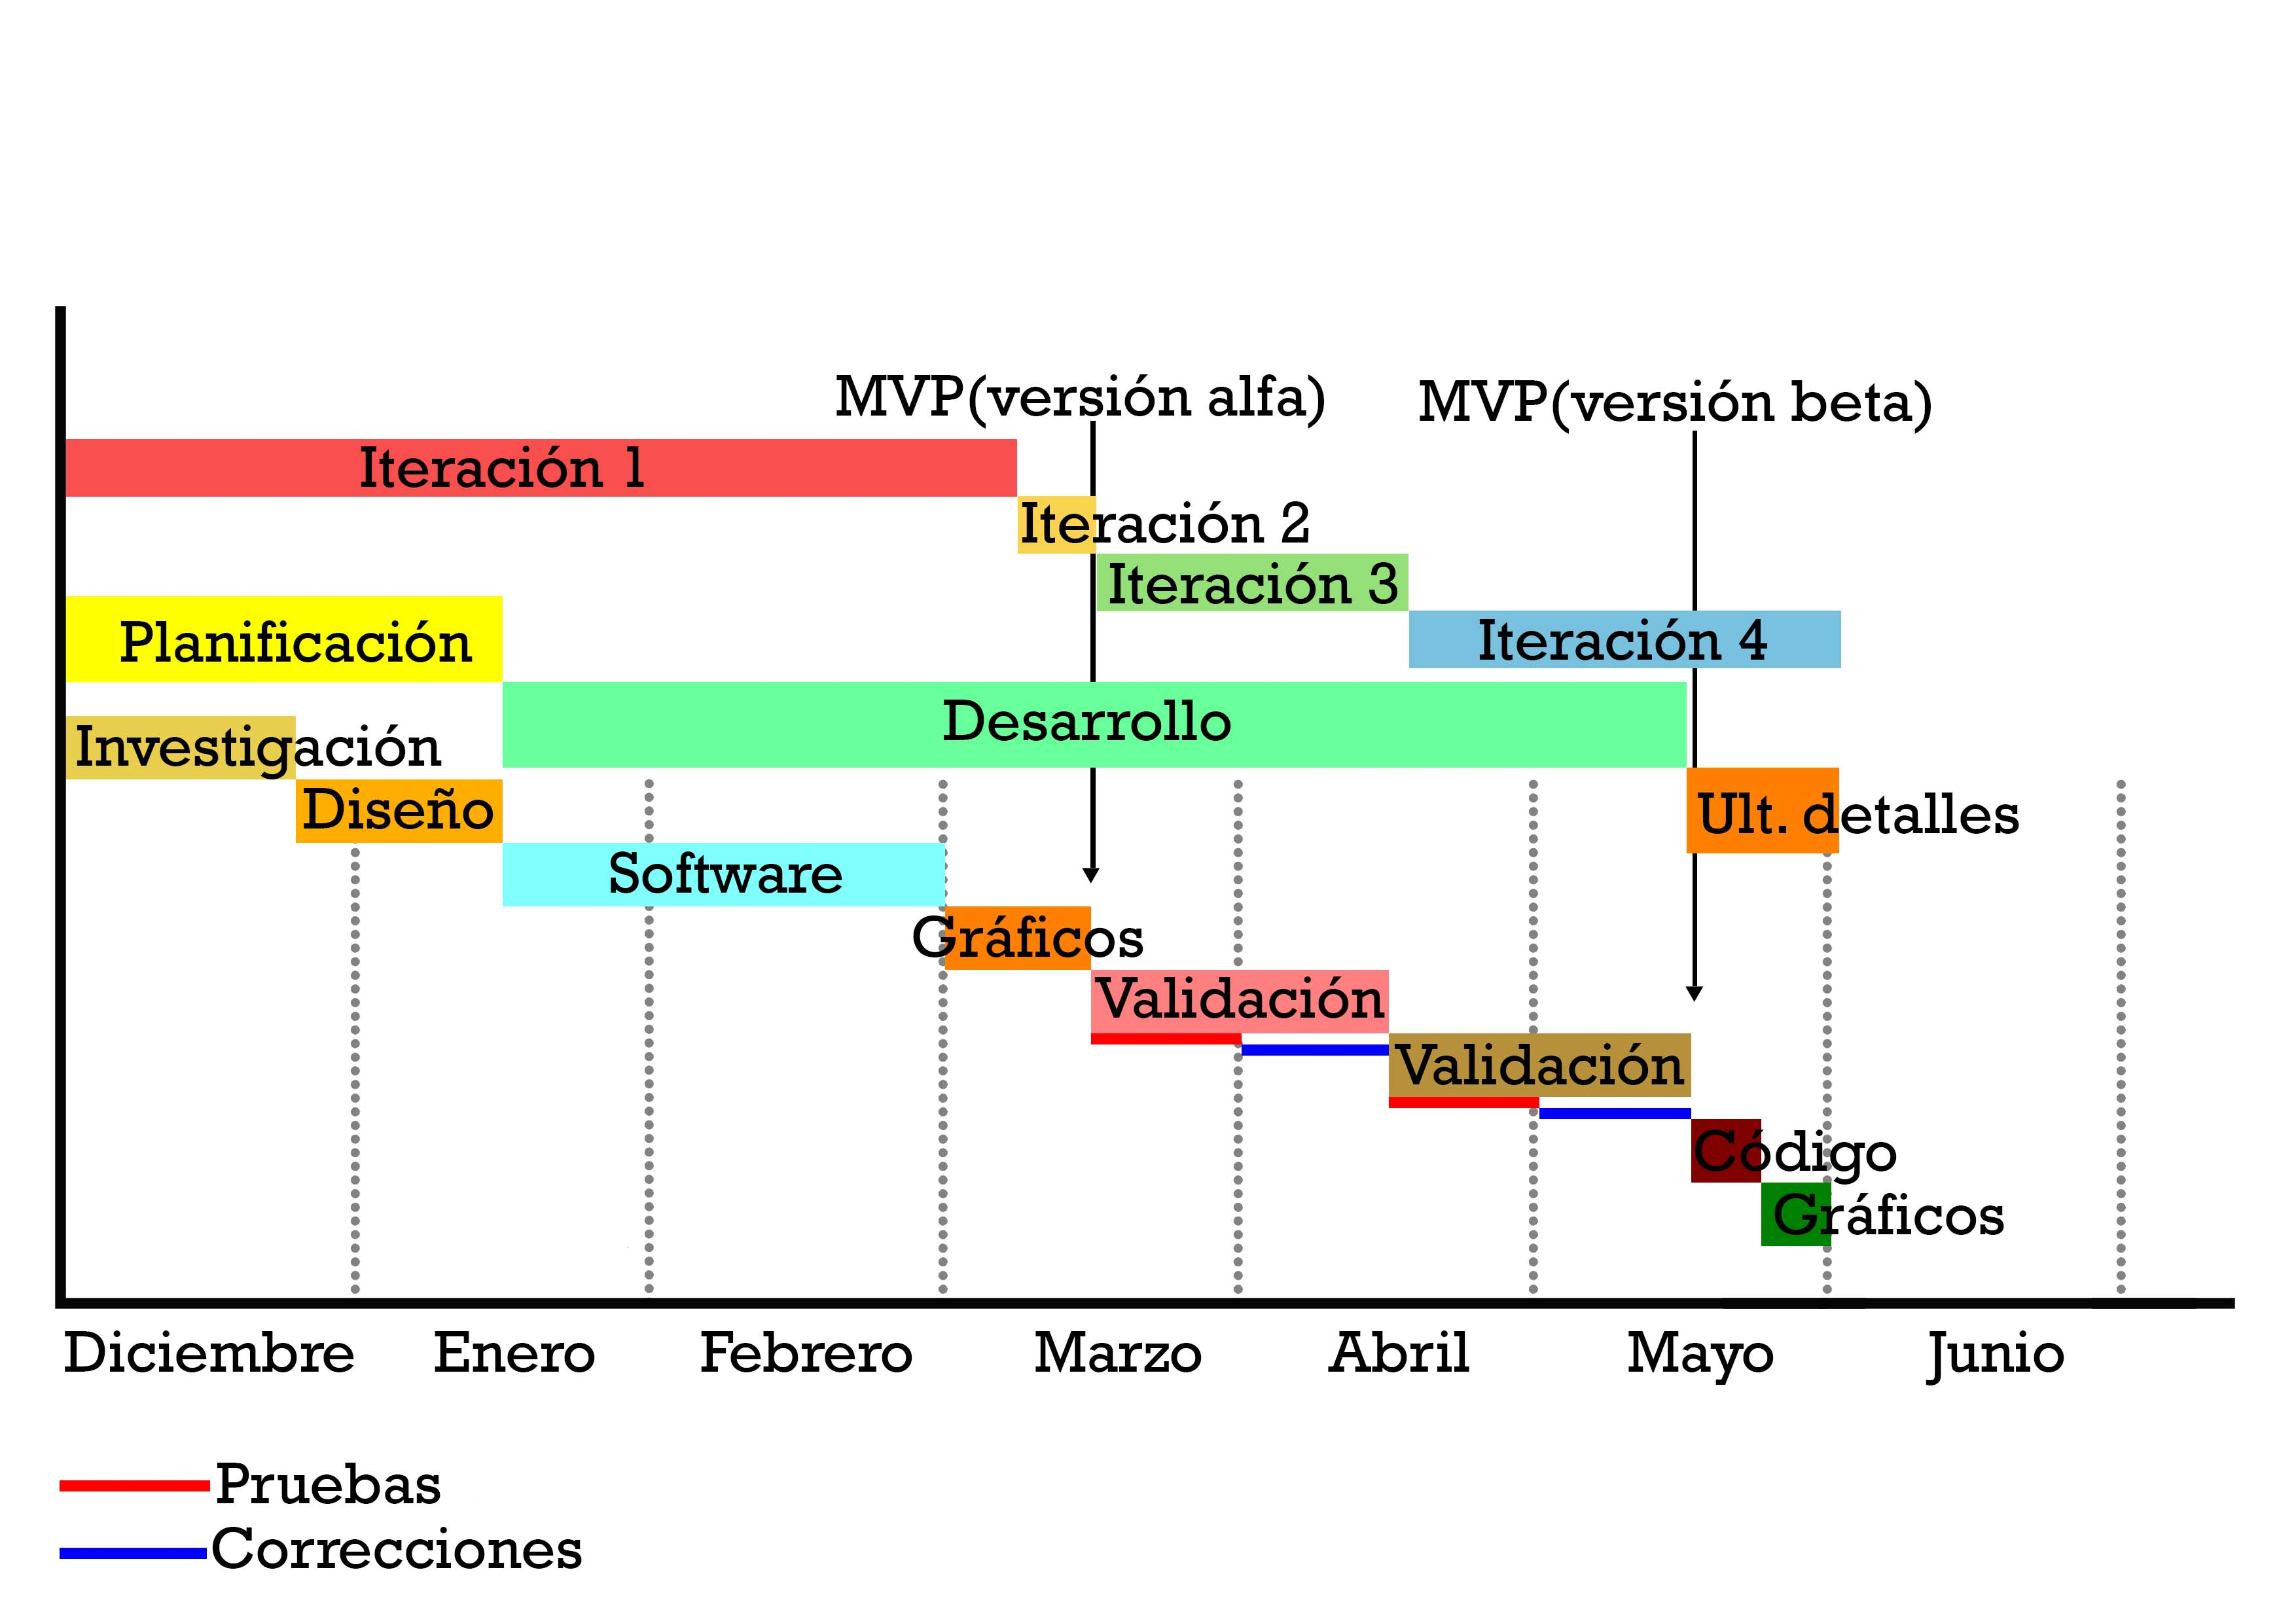
\includegraphics[scale=0.6]{imagenes/GanttDiagram.jpg}
		\caption{Diagrama de Gantt con la distribución temporal y las dependencias de las tareas}
		\label{gantt01}
	\end{center}
\end{figure}

Se utilizará la herramienta online TargetProcess \footnote{www.targetprocess.com} para disponer de un tablero virtual \textquote{Kanban} en el cual poner las tarjetas y separarlas por procesos. En este aspecto goza de más popularidad la herramienta Trello \footnote{https://trello.com/}, aunque TargetProcess es más completa y ofrece muchas opciones como filtros, métricas y otras utilidades para monitorizar el trabajo.

%\section{Producción de contenido}
%\subsection{Modelos 3D}
%Los modelos 3D a utilizar se obtendrán de sitios web que ofrezcan este tipo de recursos de forma gratuita y con licencia que permita su uso comercial. En caso de que alguno de los modelos no se encontrara se modelaría el mismo utilizando el software Blender. 
%\subsection{Música y sonidos}
%qweqwe
%\subsecion{Motor de videojuego}
%asdasda


